\begin{figure}
\centering


\tikzset{every picture/.style={line width=0.75pt}} %set default line width to 0.75pt        

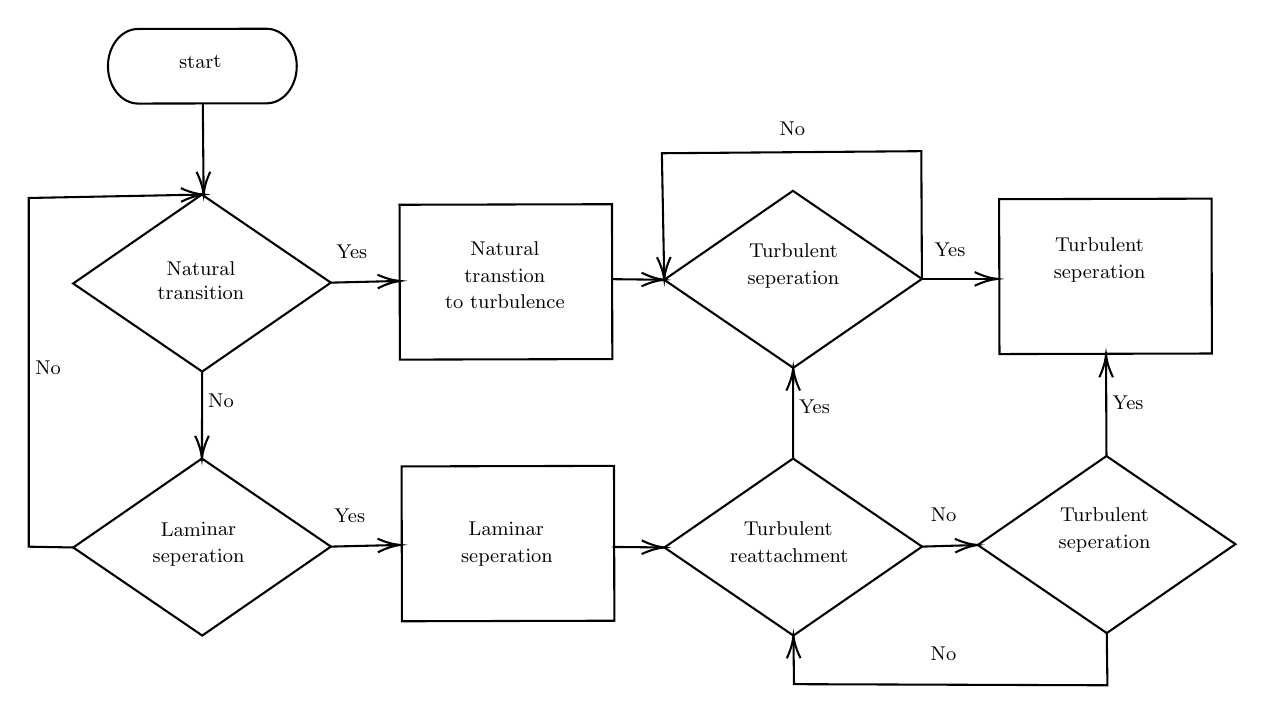
\begin{tikzpicture}[x=0.75pt,y=0.75pt,yscale=-1,xscale=1]
%uncomment if require: \path (0,734); %set diagram left start at 0, and has height of 734

%Flowchart: Terminator [id:dp7207071910268746] 
\draw   (67.63,154.62) -- (129.49,154.51) .. controls (137.52,154.5) and (144.06,162.53) .. (144.09,172.46) .. controls (144.12,182.38) and (137.62,190.44) .. (129.59,190.45) -- (67.73,190.56) .. controls (59.7,190.57) and (53.16,182.54) .. (53.13,172.61) .. controls (53.1,162.69) and (59.6,154.63) .. (67.63,154.62) -- cycle ;
%Straight Lines [id:da10986730772092312] 
\draw    (98.82,190.8) -- (99.21,232.4) ;
\draw [shift={(99.22,234.4)}, rotate = 269.47] [color={rgb, 255:red, 0; green, 0; blue, 0 }  ][line width=0.75]    (10.93,-3.29) .. controls (6.95,-1.4) and (3.31,-0.3) .. (0,0) .. controls (3.31,0.3) and (6.95,1.4) .. (10.93,3.29)   ;
%Straight Lines [id:da11218528639690684] 
\draw    (98.52,319.7) -- (98.41,359.58) ;
\draw [shift={(98.41,361.58)}, rotate = 270.15] [color={rgb, 255:red, 0; green, 0; blue, 0 }  ][line width=0.75]    (10.93,-3.29) .. controls (6.95,-1.4) and (3.31,-0.3) .. (0,0) .. controls (3.31,0.3) and (6.95,1.4) .. (10.93,3.29)   ;
%Flowchart: Decision [id:dp47636663676641755] 
\draw   (98.41,361.58) -- (160.55,404.02) -- (98.56,446.87) -- (36.41,404.44) -- cycle ;
%Flowchart: Process [id:dp0035186106511891913] 
\draw   (193.61,239.32) -- (295.96,239.05) -- (296.13,313.66) -- (193.78,313.93) -- cycle ;
%Straight Lines [id:da41405154544556755] 
\draw    (160.52,276.84) -- (191.97,276.07) ;
\draw [shift={(193.97,276.03)}, rotate = 538.61] [color={rgb, 255:red, 0; green, 0; blue, 0 }  ][line width=0.75]    (10.93,-3.29) .. controls (6.95,-1.4) and (3.31,-0.3) .. (0,0) .. controls (3.31,0.3) and (6.95,1.4) .. (10.93,3.29)   ;
%Straight Lines [id:da4839414628019604] 
\draw    (36.41,404.44) -- (14.95,404.05) -- (14.95,236.05) -- (97.22,234.44) ;
\draw [shift={(99.22,234.4)}, rotate = 538.88] [color={rgb, 255:red, 0; green, 0; blue, 0 }  ][line width=0.75]    (10.93,-3.29) .. controls (6.95,-1.4) and (3.31,-0.3) .. (0,0) .. controls (3.31,0.3) and (6.95,1.4) .. (10.93,3.29)   ;
%Straight Lines [id:da47695648438676885] 
\draw    (296.33,275.17) -- (319.14,275.44) ;
\draw [shift={(321.14,275.47)}, rotate = 180.69] [color={rgb, 255:red, 0; green, 0; blue, 0 }  ][line width=0.75]    (10.93,-3.29) .. controls (6.95,-1.4) and (3.31,-0.3) .. (0,0) .. controls (3.31,0.3) and (6.95,1.4) .. (10.93,3.29)   ;
%Flowchart: Decision [id:dp5291766920258706] 
\draw   (98.37,234.4) -- (160.52,276.84) -- (98.52,319.69) -- (36.37,277.25) -- cycle ;
%Flowchart: Process [id:dp6243738863575946] 
\draw   (194.6,365.38) -- (296.94,365.11) -- (297.11,439.72) -- (194.77,439.99) -- cycle ;
%Flowchart: Process [id:dp6109994002876044] 
\draw   (482.49,236.64) -- (584.83,236.37) -- (585,310.98) -- (482.66,311.25) -- cycle ;
%Flowchart: Decision [id:dp19310726941760736] 
\draw   (383.14,232.61) -- (445.29,275.05) -- (383.29,317.9) -- (321.14,275.46) -- cycle ;
%Flowchart: Decision [id:dp374284511592351] 
\draw   (534.21,360.39) -- (596.35,402.83) -- (534.35,445.68) -- (472.21,403.24) -- cycle ;
%Flowchart: Decision [id:dp9780902027233841] 
\draw   (383.22,361.58) -- (445.37,404.02) -- (383.37,446.87) -- (321.22,404.44) -- cycle ;
%Straight Lines [id:da6310642789542652] 
\draw    (160.55,404.02) -- (192.01,403.26) ;
\draw [shift={(194.01,403.21)}, rotate = 538.61] [color={rgb, 255:red, 0; green, 0; blue, 0 }  ][line width=0.75]    (10.93,-3.29) .. controls (6.95,-1.4) and (3.31,-0.3) .. (0,0) .. controls (3.31,0.3) and (6.95,1.4) .. (10.93,3.29)   ;
%Straight Lines [id:da12370255545736619] 
\draw    (445.29,275.05) -- (479.66,275.05) ;
\draw [shift={(481.66,275.05)}, rotate = 180] [color={rgb, 255:red, 0; green, 0; blue, 0 }  ][line width=0.75]    (10.93,-3.29) .. controls (6.95,-1.4) and (3.31,-0.3) .. (0,0) .. controls (3.31,0.3) and (6.95,1.4) .. (10.93,3.29)   ;
%Straight Lines [id:da6933448349630812] 
\draw    (296.33,404.17) -- (319.22,404.41) ;
\draw [shift={(321.22,404.44)}, rotate = 180.62] [color={rgb, 255:red, 0; green, 0; blue, 0 }  ][line width=0.75]    (10.93,-3.29) .. controls (6.95,-1.4) and (3.31,-0.3) .. (0,0) .. controls (3.31,0.3) and (6.95,1.4) .. (10.93,3.29)   ;
%Straight Lines [id:da4268759513220136] 
\draw    (445.29,275.05) -- (445,213.5) -- (320,214.5) -- (321.11,273.47) ;
\draw [shift={(321.14,275.47)}, rotate = 268.93] [color={rgb, 255:red, 0; green, 0; blue, 0 }  ][line width=0.75]    (10.93,-3.29) .. controls (6.95,-1.4) and (3.31,-0.3) .. (0,0) .. controls (3.31,0.3) and (6.95,1.4) .. (10.93,3.29)   ;
%Straight Lines [id:da994392836584868] 
\draw    (445.37,404.02) -- (470.21,403.3) ;
\draw [shift={(472.21,403.24)}, rotate = 538.3199999999999] [color={rgb, 255:red, 0; green, 0; blue, 0 }  ][line width=0.75]    (10.93,-3.29) .. controls (6.95,-1.4) and (3.31,-0.3) .. (0,0) .. controls (3.31,0.3) and (6.95,1.4) .. (10.93,3.29)   ;
%Straight Lines [id:da857618285731965] 
\draw    (383.22,361.58) -- (383.29,319.9) ;
\draw [shift={(383.29,317.9)}, rotate = 450.09] [color={rgb, 255:red, 0; green, 0; blue, 0 }  ][line width=0.75]    (10.93,-3.29) .. controls (6.95,-1.4) and (3.31,-0.3) .. (0,0) .. controls (3.31,0.3) and (6.95,1.4) .. (10.93,3.29)   ;
%Straight Lines [id:da7889844522327492] 
\draw    (534.35,445.68) -- (534.67,470.83) -- (383.67,470.29) -- (383.4,448.87) ;
\draw [shift={(383.37,446.87)}, rotate = 449.27] [color={rgb, 255:red, 0; green, 0; blue, 0 }  ][line width=0.75]    (10.93,-3.29) .. controls (6.95,-1.4) and (3.31,-0.3) .. (0,0) .. controls (3.31,0.3) and (6.95,1.4) .. (10.93,3.29)   ;
%Straight Lines [id:da8600462573826505] 
\draw    (534.21,360.39) -- (534.01,313.5) ;
\draw [shift={(534,311.5)}, rotate = 449.76] [color={rgb, 255:red, 0; green, 0; blue, 0 }  ][line width=0.75]    (10.93,-3.29) .. controls (6.95,-1.4) and (3.31,-0.3) .. (0,0) .. controls (3.31,0.3) and (6.95,1.4) .. (10.93,3.29)   ;

% Text Node
\draw (162.01,257.44) node [anchor=north west][inner sep=0.75pt]  [rotate=-359.86,xscale=0.8,yscale=0.8] [align=left] {{\small Yes}};
% Text Node
\draw (100.21,329.24) node [anchor=north west][inner sep=0.75pt]  [rotate=-359.86,xscale=0.8,yscale=0.8] [align=left] {{\small No}};
% Text Node
\draw (450.19,256.43) node [anchor=north west][inner sep=0.75pt]  [rotate=-359.86,xscale=0.8,yscale=0.8] [align=left] {{\small Yes}};
% Text Node
\draw (16.92,313.42) node [anchor=north west][inner sep=0.75pt]  [rotate=-359.86,xscale=0.8,yscale=0.8] [align=left] {{\small No}};
% Text Node
\draw (359.18,257.04) node [anchor=north west][inner sep=0.75pt]  [rotate=-359.86,xscale=0.8,yscale=0.8] [align=left] {\begin{minipage}[lt]{43.095000000000006pt}\setlength\topsep{0pt}
\begin{center}
{\small Turbulent \ }\\{\small seperation }
\end{center}

\end{minipage}};
% Text Node
\draw (86.09,166.8) node [anchor=north west][inner sep=0.75pt]  [font=\small,rotate=-358.05,xscale=0.8,yscale=0.8] [align=left] {{\small start}};
% Text Node
\draw (61.17,265.54) node [anchor=north west][inner sep=0.75pt]  [font=\small,rotate=-359.86,xscale=0.8,yscale=0.8] [align=left] {\begin{minipage}[lt]{66.671875pt}\setlength\topsep{0pt}
\begin{center}
{\small Natural transition }\\
\end{center}

\end{minipage}};
% Text Node
\draw (72.55,391.21) node [anchor=north west][inner sep=0.75pt]  [rotate=-359.86,xscale=0.8,yscale=0.8] [align=left] {\begin{minipage}[lt]{43.095000000000006pt}\setlength\topsep{0pt}
\begin{center}
{\small Laminar}\\{\small seperation }
\end{center}

\end{minipage}};
% Text Node
\draw (209.74,255.99) node [anchor=north west][inner sep=0.75pt]  [rotate=-359.86,xscale=0.8,yscale=0.8] [align=left] {\begin{minipage}[lt]{62.591875pt}\setlength\topsep{0pt}
\begin{center}
{\small Natural transtion}\\{\small  to turbulence}
\end{center}

\end{minipage}};
% Text Node
\draw (222.02,391.11) node [anchor=north west][inner sep=0.75pt]  [rotate=-359.86,xscale=0.8,yscale=0.8] [align=left] {\begin{minipage}[lt]{40.831875000000004pt}\setlength\topsep{0pt}
\begin{center}
{\small Laminar }\\{\small seperation}
\end{center}

\end{minipage}};
% Text Node
\draw (160.99,384.51) node [anchor=north west][inner sep=0.75pt]  [rotate=-359.86,xscale=0.8,yscale=0.8] [align=left] {{\small Yes}};
% Text Node
\draw (507.57,254.06) node [anchor=north west][inner sep=0.75pt]  [rotate=-359.86,xscale=0.8,yscale=0.8] [align=left] {\begin{minipage}[lt]{41.426875pt}\setlength\topsep{0pt}
\begin{center}
{\small Turbulent \ }\\{\small seperation}
\end{center}

\end{minipage}};
% Text Node
\draw (351.6,390.97) node [anchor=north west][inner sep=0.75pt]  [rotate=-359.86,xscale=0.8,yscale=0.8] [align=left] {\begin{minipage}[lt]{52.615pt}\setlength\topsep{0pt}
\begin{center}
{\small Turbulent \ }\\{\small reattachment }\\
\end{center}

\end{minipage}};
% Text Node
\draw (375.51,198.09) node [anchor=north west][inner sep=0.75pt]  [rotate=-359.86,xscale=0.8,yscale=0.8] [align=left] {{\small No}};
% Text Node
\draw (509.09,384.2) node [anchor=north west][inner sep=0.75pt]  [rotate=-359.86,xscale=0.8,yscale=0.8] [align=left] {\begin{minipage}[lt]{43.095000000000006pt}\setlength\topsep{0pt}
\begin{center}
{\small Turbulent }\\{\small seperation }
\end{center}

\end{minipage}};
% Text Node
\draw (448.33,451.37) node [anchor=north west][inner sep=0.75pt]  [rotate=-359.86,xscale=0.8,yscale=0.8] [align=left] {{\small No}};
% Text Node
\draw (384.9,332.18) node [anchor=north west][inner sep=0.75pt]  [rotate=-359.86,xscale=0.8,yscale=0.8] [align=left] {{\small Yes}};
% Text Node
\draw (448.37,384.05) node [anchor=north west][inner sep=0.75pt]  [rotate=-359.86,xscale=0.8,yscale=0.8] [align=left] {{\small No}};
% Text Node
\draw (536.01,330.44) node [anchor=north west][inner sep=0.75pt]  [rotate=-359.86,xscale=0.8,yscale=0.8] [align=left] {{\small Yes}};


\end{tikzpicture}


\caption{Boundary layer flowchart} 
\label{fig:M1}
\end{figure}